\chapter[Second Law and Entropy]{Second Law of Thermodynamics and  Entropy}
\label{chapter:second_law}


%\section*{Objectives}
%
%\begin{objectives}
%
%\item State and use the definitions of microstates, macrostates,
%  and multiplicity.  Understand the connection between multiplicity
%  and probability.
%
%\item Calculate the multiplicity of an Einstein solid or two
%  coupled Einstein solids.  Determine the temperature of an Einstein
%  solid.
%
%\item Understand the implications of the second law of
%  thermodynamics to heat flow and irreversibility.  Describe the
%  second law in terms of probability, multiplicity, and entropy. 
%
%\item State the definition of temperature and show that this
%  definition is consistent with the Clausius statement of the second
%  law.
%
%\end{objectives}

%\section{Introduction}

In this chapter we will discuss one of the most significant
developments in the history of science --- the development of a {\em
  statistical} theory of thermodynamics.  Here is the question: if a
chunk of ice, or a glass of water, or an air-filled balloon is composed of
$10^{22}$ or $10^{23}$ molecules, isn't it necessary to describe the
dynamics of each individual molecule?  To determine the force on each
molecule and solve Newton's second law to figure out its motion?  The
answer is no, thankfully.  Instead, we can treat each of these
molecules as though they are behaving randomly, and recover all the
results of thermodynamics from a probabilistic treatment.

%In this theory, the
%behavior that we observe happens because it is the most likely
%scenario.  At first glance, this might seem unreasonable; after all,
%the fact that a state is less likely doesn't mean that it can't
%happen, correct?  Yes, but when we consider systems with $10^{23}$
%molecules in it, it turns out that the more likely states are {\bf
%  overwhelmingly}\footnote{The word ``overwhelming'' doesn't even
%  begin to describe just how much more probably the most probable
%  states are.  If we said that these states are much, much, much,
%  much, much, much, ... more probable, we'd have to spend several
%  decades repeating the word ``much'' to begin to get even a hint of
%  the magnitude of the probability here.} more likely and the less
%likely states are {\bf overwhelmingly} less likely.  In fact, the odds
%are so {\bf ridiculously} weighted that we will say that the more
%likely states ``always'' happen and that the less likely states
%``never'' happen.

The importance of this statistical approach cannot be overstated.
The idea that we can treat thermodynamic systems probabilistically
led to a revolution in scientific thought that ranks up there
with Newton's development of classical physics, Pasteur's development
of germ theory of disease, Einstein's theory of relativity, and
the development of quantum mechanics (which you'll see in PHYS 212).

We will introduce statistical mechanics by revisiting the basic phenomenon
of heat flow, the spontaneous thermal energy transfer from hotter objects
to colder objects.  The direction of the heat flow is determined by what
is known as the {\it second law of thermodynamics.}  We can derive the
second law of thermodynamics from probability arguments; essentially,
thermal energy flow is dictated by moving from an improbable to a
probable situation.  Entropy is introduced as a measure of probability.
And along the way to understanding the second law, we will provide a
general definition of temperature.

\section{Heat Flow Revisited}

Consider the following process, illustrated in
Fig.~\ref{fig:paradigmatic_process}: a hot piece of metal is placed
into a container holding cold water.  As time passes, thermal energy
flows from the metal to the water, making the metal colder and the
water warmer.  Eventually, the two are at the same temperature and no
more thermal energy is transferred.  This is {\it heat\/}: the
spontaneous thermal energy transfer due to the temperature difference,
as we identified in section~\ref{section:heat}.

\begin{figure}
\begin{center}
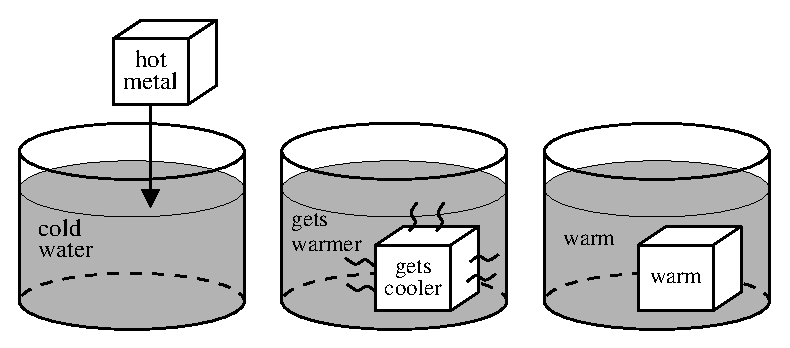
\includegraphics[width=4.6in]{second_law_and_entropy/paradigm}
\caption{A hot piece of metal is placed into cold water.  Thermal
  energy is transferred from the hot metal to the cold water until
  they are in thermal equilibrium.}
\label{fig:paradigmatic_process}
\end{center}
\end{figure}

In a heat flow scenario, such as this one, the first law of
thermodynamics states that energy is conserved, and so we must have
\begin{equation}
\Delta E_\text{therm,water} = -\Delta E_\text{therm,metal}.
\end{equation}
However, energy conservation would be equally well satisfied if the
heat flowed the other way.  Imagine putting the hot metal into cold
water and finding that the metal becomes increasingly hotter while the
water becomes increasingly cooler, beginning to freeze.  Absurd!  This
is never observed to happen.  And yet it would be perfectly consistent
with the first law of thermodynamics.

What this process illustrates is that there must be an additional law
of nature involved that determines the direction of heat flow.  In a
fit of creativity, physicists decided to call this the {\it second}
law of thermodynamics.  There are many equivalent ways to state the
second law.  We will begin with the {\it Clausius statement} of the
second law, since it is the most intuitive.

\boxittext{
{\sc 2nd Law of Thermodynamics (Clausius):}\\  \raggedright
Heat cannot flow spontaneously from a material at lower temperature to
a material at higher temperature.
}

Let's examine this.  First, note that the law is, at this point,
empirical, which means it is a statement about the observed behavior
of nature.  The second law rules out the absurd scenario whereby heat
flowed from the cold water to the hot metal.  But, note that the
second law makes no statement about whether the heat will actually
flow from the metal to the water.  According to the second law, this heat
flow is allowed, but not required.  That is exactly what we want from
a general law, since after all the metal and the water may or may not
be thermally coupled.

Temperature plays a crucial role in the second law, since the question
of whether heat is allowed to flow from $A$ to $B$ or instead from $B$
to $A$ is answered by the temperatures $T_A$ and $T_B$.  Temperature
plays the role of nature's traffic cop, enforcing thermodynamic
``one-way streets.''\footnote{However, nature needs no traffic court
  since its one-way streets, like its speed limit, are
  self-enforcing.}  The primary topic of this chapter is the
explanation of why temperature plays this role.

Another interesting aspect of the second law is the phenomenon of {\it
irreversibility.}  Many processes in nature are reversible.  A movie of
the flight of a ball thrown straight up into the air, turning around and
coming back down, looks the same whether played forward or backward.
This is because Newton's law are {\it reversible} as long as friction
is negligible.  But once heat flows from the hot metal to the cold
water, it will never spontaneously  flow back again.  A movie of the
process (with some thermometers used to make the temperature visible)
would look different played backward versus forward.  Physicists believe
the second law is the origin of any irreversibility observed in nature,
which is to say, the second law of thermodynamics plays a crucial role
in determining the direction of time flow.

Interestingly, the second law is unique among laws of physics.  Most
laws are simply inferred from the behavior of nature.  We don't know
why energy conservation happens; we just know it does.  The second law
is different because we can essentially derive it.  We know {\it why}
it happens.  It is ultimately a statement about probability: thermal
energy flows spontaneously from hotter objects to colder objects
because that brings the system to a state with a more 
likely arrangement of energy.  

The rest of this chapter is concerned with expanding our probabilistic
understanding of the second law and temperature.  
% For this purpose, we
% will need to develop the concepts of microstates, macrostates, and
% multiplicity. 

\section{Microstates, Macrostates, and Multiplicity}

To explain how probabilities work in thermodynamics --- and ultimately
to explain entropy and how it relates to the second law of
thermodynamics --- it is necessary to discuss some fundamental
concepts of probability.  We start with definitions of 
{\em microstates} and {\em macrostates}:

\boxittext{
A {\it macrostate} is a specification of the macroscopic state of the
system.  For example, the pressure, temperature, and number of moles
of an ideal gas would specify a macrostate.
\bigskip

A {\it microstate} is the detailed specification of the microscopic
state of the system.  In the ideal gas example, the microstate would
be precise values for the position and velocity of every single
molecule.
}

A macrostate can have many microstates associated with it.  In the
ideal gas example, there are many possible arrangements of the
molecules that are consistent with having, say, one mole of gas with
atmospheric pressure and room temperature.  This brings us to
multiplicity:

\boxittext{
The {\it multiplicity} $\Omega$ of a macrostate is the number of
microstates associated with that macrostate. 
}

Let's explore these ideas with a specific example: a pair of six-sided
dice, one red and one green.\footnote{Having dice of the same color
  wouldn't change anything.  We just use different colors to help
  label the dice.}  There are 36 possible outcomes of rolling these
dice, listed in Table~\ref{table:paradise}, and the sum of the two
dice can be any number between two and twelve.  Not every sum is
equally probable, however.   If you roll the dice many times, you will
notice you get a sum of seven much more often than, say, a sum of
twelve.

The 36 possible outcomes are the microstates.  The red dice showing
`5' and the green die showing `3' would be a particular microstate
(labeled 5-3 in Table~\ref{table:paradise}).  The sum of the dice,
eight in this case, represents a macrostate.  Notice that there are
many ways to roll a sum of eight; or stated another way, there are
multiple microstates associated with the macrostate `8.'  The number
of ways to roll an `8' is the multiplicity $\Omega$.  Looking at
Table~\ref{table:paradise}, we see there are five different ways to
roll an `8', so the multiplicity $\Omega =5$.

The multiplicity of a macrostate is useful to know because it tells us
the probability of obtaining that particular macrostate.  Each of the
36 microstates for a pair of dice is equally likely.  The reason that
a sum of seven is a more likely outcome than a sum of twelve is not
because 4-3 is more likely than 6-6 (it's not!), rather, there are
more ways to roll a `7.'

Now let's come back to physics.  The macrostate of a collection of
molecules  could be defined in terms of the number of particles and
the amount of energy $E_\text{therm}$ they have.  A microstate would
correspond to a particular arrangement of the energy among the
molecules.  Since there are many possible ways to arrange the energy
among the molecules, there are many microstates associated with this
macrostate.  The number of possible ways to arrange the given amount
of energy would then be the multiplicity $\Omega$.

\begin{table}
\begin{center}
\begin{tabular}{clcl}
\hline\hline
sum & rolls (red die--green die) & $\Omega$ & probability \\
\hline
2 & 1-1 & 1 & 1/36 \\
3 & 1-2 \quad 2-1 & 2 & 2/36 = 1/18 \\
4 & 1-3 \quad 2-2 \quad 3-1 & 3 & 3/36 = 1/12 \\
5 & 1-4 \quad 2-3 \quad 3-2 \quad 4-1 & 4 & 4/36 = 1/9 \\
6 & 1-5 \quad 2-4 \quad 3-3 \quad 4-2 \quad 5-1 & 5 & 5/36 \\
7 & 1-6 \quad 2-5 \quad 3-4 \quad 4-3 \quad 5-2 \quad 6-1 & 6 & 6/36 = 1/6 \\
8 & 2-6 \quad 3-5 \quad 4-4 \quad 5-3 \quad 6-2 & 5 & 5/36 \\
9 & 3-6 \quad 4-5 \quad 5-4 \quad 6-3 & 4 & 4/36 = 1/9 \\
10 & 4-6 \quad 5-5 \quad 6-4 & 3 & 3/36 = 1/12 \\
11 & 5-6 \quad 6-5 & 2 & 2/36 = 1/18 \\
12 & 6-6 & 1 & 1/36 \\
\hline\hline
\end{tabular}
\caption{The 36 possible results from rolling a pair of dice (one
  red, one green).}
\label{table:paradise}
\end{center}
\end{table}
  
To go from multiplicity to probability we need one more piece of
information.  In the case of the dice, each of the 36 possible
outcomes was equally likely, assuming that the dice were fair,
returning each of the six values with equal probability.  Does this
apply as well for our system of $N$ particles sharing a total energy
$E_\text{therm}$?  In general, we cannot prove this, but to make
progress we will assume that it is true.

\boxittext{\raggedright
{\sc The Fundamental Assumption of Statistical Mechanics:}\\
All of a system's accessible microstates are equally likely.
}

``Accessible microstates'' here means simply those which are allowed by
energy conservation.  The motivation for this assumption is that
whatever the specific dynamics are, however the molecules are
colliding and sloshing energy back and forth among each other, they
eventually visit every possible state allowed by energy conservation.
So a sequence of snapshots of the system would look like randomly
selected examples of possible microstates.   In the end, nature has
confirmed that starting with the fundamental assumption leads to
predictions that match experiments extremely well.  Now we shall see
what the fundamental assumption buys us.

\section{Einstein Solid}

We now develop the ideas of the previous section in the context of a
specific model.  The simplest model to work with, it turns out, is not
the ball-spring model or the ideal gas, but rather a variation of the
ball-spring solid called the Einstein solid.  Experiments on very cold
metals showed that their specific heats could fall well below the
value $3R$, suggesting something not contained in the ball-spring
model was occurring at low temperatures.  Einstein showed that a
quantum mechanical version of the ball-spring model could explain this
result.\footnote{The complete description of very cold metals requires
  an additional modification, worked out by a Dutch physicist named
  Peter Debye.  We will not consider the Debye theory here.}  To
begin, notice that a three-dimensional oscillator, such as the
molecule in the ball-spring model, can be written as a sum of three
independent, one-dimensional oscillators:
\begin{align}
E_\text{ball} &= \bigl(\textstyle\frac{1}{2} m v_x^2 + \frac{1}{2} m v_y^2 
+ \frac{1}{2} m v_z^2\bigr) +
\bigl(\textstyle\frac{1}{2} k_{sp} x^2
+ \frac{1}{2} k_{sp} y^2 + \frac{1}{2} k_{sp}z^2\bigr)
\nonumber\\[1.5ex]
 &= \bigl(\textstyle\frac{1}{2}mv_x^2+
   \frac{1}{2}k_{sp}x^2\bigr)
+\bigl(\textstyle\frac{1}{2}mv_y^2+\frac{1}{2}k_{sp}y^2\bigr)
+\bigl(\textstyle\frac{1}{2}mv_z^2+\frac{1}{2}k_{sp}z^2\bigr)
\end{align}
In the second grouping, each term in parentheses is an oscillator
moving in one particular direction and independent of the motion in
the other perpendicular directions.  Thus a set of $N$ molecules in
the ball-spring model is equivalent to $3N$ one-dimensional
oscillators.  In what follows we will be working primarily with the
one-dimensional oscillators so we let $N$ represent the number of
oscillators instead of the number of molecules.  The number of
molecules is then $N/3$.

Einstein proposed to treat the one-dimensional oscillators quantum
mechanically, which should be appropriate when the temperature is
low enough.  We will not discuss quantum mechanics here --- that is a
topic for PHYS 212 --- but we will summarize the main results of interest
to us.  The energy levels of the quantum harmonic oscillator are not
continuous but rather discrete (or {\it quantized\/}).  This is
illustrated in Fig.~\ref{fig:qho}.  At very low energies we cannot
vary the oscillator energy up or down by arbitrarily small amounts,
but rather can only add energy in discrete chunks.  Furthermore, for
the quantum harmonic oscillator, these energy levels are equally
spaced.  Therefore we can write the energy level of an oscillator as
\begin{equation}
E_\text{osc} = E_0 + n\epsilon \qquad
\text{where $n=0$, 1, 2, 3, \dots}
\end{equation}
Here $E_0$ is the lowest energy level possible, and we may increase
the energy by adding an integer number of ``energy units'' of size
$\epsilon$. 

\begin{figure}
\begin{center}
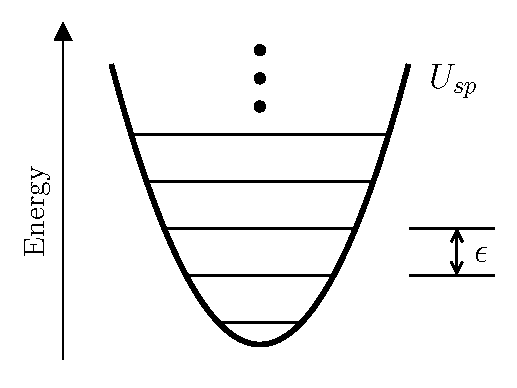
\includegraphics[width=2in]{second_law_and_entropy/qho}
\caption{The quantum harmonic oscillator has discrete energy levels,
  shown as horizontal lines.  The energy difference between successive
  levels is $\epsilon$.}
\label{fig:qho}
\end{center}
\end{figure}

Now consider a system of two oscillators, with a total energy of three
``energy units.''  These oscillators bounce energy back and forth and
so one of the oscillators may have at a given instant anywhere from
zero to all three of the energy units.  Let $n_1$ be the number of
energy units that the first oscillator has, and $n_2$ the number of
energy units for the second oscillator.  Specifying $n_1$ and $n_2$
determines a particular microstate.  The total energy of three units
implies $n_1+n_2=3$, so the possible microstates, written as
$(n_1,n_2)$, are
\[
(3,0), \quad (2,1), \quad (1,2), \quad (0,3).
\]
Evidently, the multiplicity of the macrostate with two oscillators and
a total of three energy units is $\Omega =4$.  That is, there are four
different microstates with this total energy.

\begin{example}{Three oscillators, two energy units}
  Write down all the microstates for a system of three oscillators and
  a total of two energy units, and determine the multiplicity.
  \solution 
  For microstates written as $(n_1,n_2,n_3)$, we need to have
  $n_1+n_2+n_3=2$, so the possible microstates are
\[
(2,0,0),\quad(0,2,0),\quad(0,0,2),\quad
(1,1,0),\quad(1,0,1),\quad(0,1,1),
\]
and the multiplicity $\Omega=6$.
\label{example:multiplicity}
\end{example}

It is feasible to determine the multiplicity directly by counting the
microstates when the number of oscillators and energy units is small.
But this becomes unwieldy very quickly as the number  of oscillators
and energy units is increased.  Fortunately, we can derive the general
result for $N$ oscillators and $q$ total energy units, which is
\begin{equation}
\Omega = \frac{(q+N-1)!}{q!\;(N-1)!}.
\label{eq:Einstein_multiplicity}
\end{equation}
The factorial function is defined as $n!=n(n-1)(n-2)\cdots 2\cdot 1$.
For example, $5!=5\cdot 4\cdot 3\cdot 2\cdot 1=120$.  A special
case is the factorial of the number zero:  by definition, 
$0!=1$.  The meaning of $n!$ is that it is the number of
distinct ways to order $n$ objects.  The number of ways to order zero
objects is taken to be 1.

\begin{example}{Checking the multiplicity formula.}
Verify the Einstein solid multiplicity formula,
Eq.~(\ref{eq:Einstein_multiplicity}), for the cases of two oscillators
with three energy units and three oscillators with two energy units.
\solution
For two oscillators and three energy units ($N=2$ and $q=3$) the
multiplicity formula gives
\begin{equation}
\Omega = \frac{(3+2-1)!}{3!\;(2-1)!} = \frac{4!}{3!\;1!} =
\frac{24}{6\cdot 1} = 4,
\end{equation}
which matches our result above.  For the second case, $N=3$ and $q=2$,
giving
\begin{equation}
\Omega = \frac{(2+3-1)!}{2!\;(3-1)!} = \frac{4!}{2!\;2!} = \frac{24}{2^2}
= 6,
\end{equation}
verifying the second case.
\end{example}

Factorials become very large very quickly.  For example, $100!\approx
10^{157}$, which is an amazingly large number.  An Einstein solid with
100 oscillators and 200 energy units has a multiplicity $\Omega =
2.8\times 10^{82}$.  Now you can appreciate having
Eq.~(\ref{eq:Einstein_multiplicity}) to work with instead of counting
all possible microstates.  And imagine how large the result would be
for Avogadro's number of oscillators!

\section{Coupled Einstein Solids}

Our original goal was to understand heat flow.  That is, why thermal
energy spontaneously goes from hotter objects to colder objects.  To
that end, we will now consider two Einstein solids, solid $A$ with a
number $N_A$ oscillators and $q_A$ energy units, and solid $B$ with
$N_B$ oscillators and $q_B$ energy units.  If solids $A$ and $B$ are
brought into thermal contact, then they will be able to pass energy
units back and forth while maintaining a fixed total
$q_\text{tot}=q_A+q_B$.  But which way will the energy go, on average?  And
when will it come to thermal equilibrium?  Let us try to address these
questions. 

Once the two Einstein solids are thermally coupled and exchanging
energy, $A$ and $B$ should be regarded as {\it subsystems} of the
combined system.  For a particular division of energy among the two
subsystems, we have a multiplicity $\Omega_A$ that depends on $N_A$
and $q_A$, and a multiplicity $\Omega_B$ that depends on $N_B$ and
$q_B$.  

How do we calculate the combined multiplicity of the system?  If you
have three pairs of pants and five shirts, then you have $3\cdot 5=15$
possible combinations you can make, at least in polite company.
Similarly, subsystem $A$ may be in any of the number $\Omega_A$
microstates and subsystem $B$ in any of $\Omega_B$ microstates, so the
number of paired microstates we can make is the product $\Omega_{AB} =
\Omega_A\Omega_B$.  This is the combined multiplicity of the system.

Let's consider a specific case.  Let $N_A=3$ and $N_B=3$, and
$q_\text{tot}=q_A+q_B=6$.  The two systems may divide up the six energy
units a variety of ways, as shown in Table~\ref{table:two_systems}.
For each choice, the multiplicities $\Omega_A$ and $\Omega_B$ and the
combined multiplicity $\Omega_{AB}$ are given.  Note that the most
probable arrangement of energy, the one with the largest multiplicity,
is the one with three energy units in each subsystem.  If subsystem
$A$ started with zero energy units and subsystem $B$ with six units,
then simple random energy exchanges would move the coupled systems
toward the more probable state with $q_A=q_B=3$.  This is a clue about the
origin of the second law.

\begin{table}
\begin{center}
\begin{tabular}{ccrrr}
\hline\hline
$q_A$ & $q_B$ & \qquad $\Omega_A$ & $\Omega_B$ & \qquad $\Omega_{AB}$ \\
\hline
0 & 6 & 1 & 28 & 28 \\
1 & 5 & 3 & 21 & 63 \\
2 & 4 & 6 & 15 & 90 \\
3 & 3 & 10 & 10 & 100 \\
4 & 2 & 15 & 6 & 90 \\
5 & 1 & 21 & 3 & 63 \\
6 & 0 & 28 & 1 & 28 \\
\hline\hline 
\end{tabular}
\caption{Possible macrostates for system $A$ and $B$ sharing six units
  of energy, with $N_A=3$ and $N_B=3$.}
\label{table:two_systems}
\end{center}
\end{table}

From Table~\ref{table:two_systems} we see that the most probable
situation is only slightly more probable than the other possibilities.
This changes dramatically as the system size is increased.  In
Fig.~\ref{fig:multiplicity_with_size} we plot the combined
multiplicity as a function of $q_A$ for various numbers of oscillators
and energy units.  As the figure shows, when the numbers become
larger, say in the thousands, the multiplicity function becomes 
sharply peaked.  Some particular division of energy between
the two subsystems is vastly, hugely, awesomely, mind-bogglingly more
probable\footnote{I.e., it isn't just a little more probable, it is a
  {\bf lot} more probable.} than all others.  This we identify as the
equilibrium division of energy.  Now imagine what occurs when you
approach Avogadro's number of energy units.  The multiplicity function
becomes completely sharp.  There is some particular division of the
energy between subsystems $A$ and $B$ that is ridiculously, 
overwhelmingly, staggeringly\footnote{``\dots vastly, hugely,
  awesomely, mind-bogglingly, ...'' and that doesn't even begin to cover it!}
more probable than any other.

\begin{figure}
\begin{center}
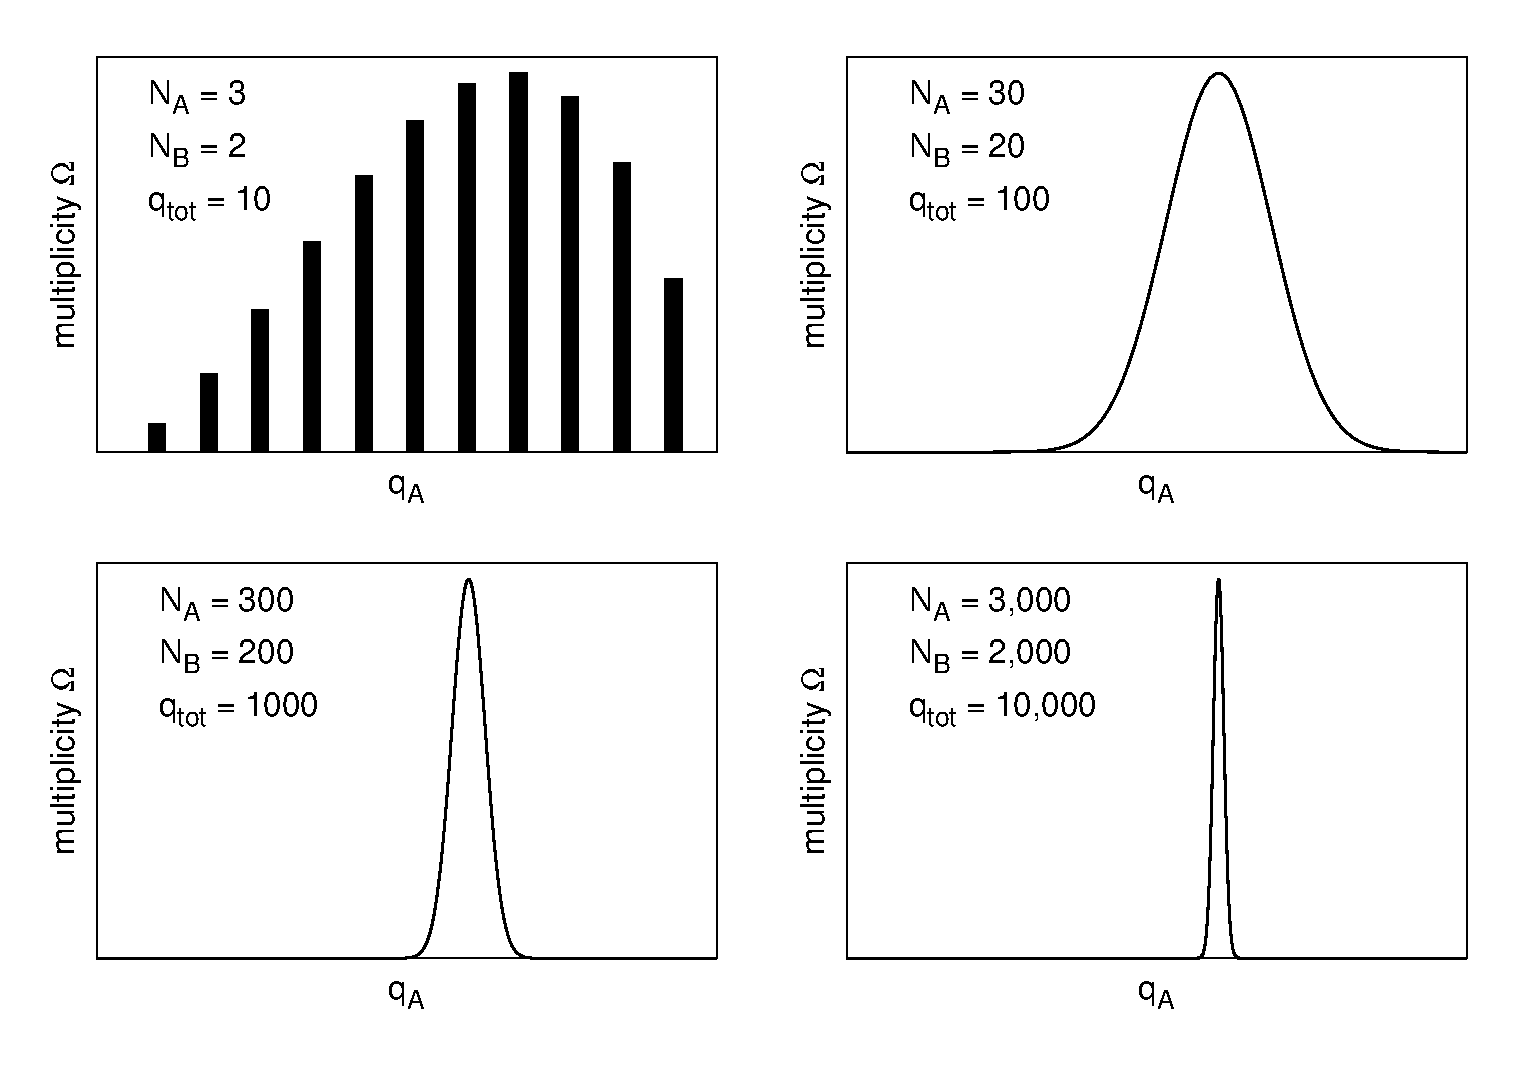
\includegraphics[width=5in]{second_law_and_entropy/multiplicity_with_size.eps}
\caption{Plots of the multiplicity as a function of $q_A$ for a
  variety of system sizes.  Note that $q_B$ is determined by
  $q_A+q_B=q_\text{tot}$.} 
\label{fig:multiplicity_with_size}
\end{center}
\end{figure}

Now we have the probabilistic origin of the second law.  Subsystems
$A$ and $B$, before they are thermally coupled, can be prepared with
any thermal energy we would like.  We made the metal object hot and
the water cold before plunging the metal into the water.  But once the
subsystems are thermally coupled, they will move from whatever
division of energy they started with toward the maximally probable
arrangement of energy for the coupled system.  They are irresistibly
led to it by essentially random exchanges of energy between the
subsystems.  The energy transferred along the way is what we had
previously identified as heat.

To summarize:

\boxittext{
The second law of thermodynamics is a result of a system prepared in
an improbable initial state then moving to a vastly more probable
final state.}
\break
{\bf This is an incredibly important result!!!!}  With this
statement, we don't have to worry at all about the detailed,
Newtonian mechanics of the (many, many) individual molecules or
atoms in a solid, liquid or gas.  We treat all the motion as though
it is random and then simply figure out the probabilities.  

\section{Entropy}

Entropy is part of the title of the chapter; perhaps it is time we
introduced it.  The fact is, we have already been discussing the
entropy, because entropy is simply the multiplicity cast into a more
convenient form, by means of a logarithm.  We define entropy as
\begin{equation}
S = k_B\ln\Omega.
\label{eq:entropy_def}
\end{equation}
The factor of Boltzmann's constant plays little role here, apart from
giving entropy units (which are J/K).\footnote{By the way, Boltzmann
was the one who realized that the second law had a probabilistic origin,
and Eq.~(\ref{eq:entropy_def}) is engraved on his tombstone.  Check it
out if you're ever in Vienna.}  The logarithm is a monotonic function,
which means that the larger $\Omega$ gets, the larger $S$ gets.  So being
the most probable state is the same as being the highest entropy state.
This is a really important statement, so important that we will elevate
it to box-dom:

\boxittext{Entropy is a measure of probability:  the more probable a
state, the higher its entropy.}
\break
Entropy is often incorrectly described as a measure of the disorder
of a system.  This is simply not true; entropy is measure of
probability and probability only.  It {\bf is} true that higher
entropy states are often more disordered than lower-entropy states,
but this is not always true; there are many examples
%have been several experiments recently 
of systems that become {\bf more} ordered as their
entropy increases.

We can now write the second law of thermodynamics rather concisely as
a statement of probability, given in the boxed statement at the end of
the previous section:
\begin{equation}
\Delta S_\text{total} \geq 0. \qquad\text{(Entropic version of 2nd law)}
\end{equation}
Starting from some initial state that is not the maximum entropy
state, the combination of all our subsystems will exchange thermal
energy and move spontaneously toward the maximum entropy state.  And
for large systems, it moves irreversibly: there is a negligibly small
probability of moving away from the maximum entropy state
(think about the sharply peaked multiplicity).

Note that the entropic form of the second law refers to the {\bf total}
entropy of a system, i.e., the {\bf total} entropy cannot decrease.
But the entropy of part of a system {\bf can} decrease.  So, for
instance, it is very possible to have a chemical reaction where
the stuff inside your beaker ends up with a lower entropy,
as long as there is a corresponding increase in entropy somewhere
else (most likely in the air around the beaker whose entropy
increases when heated up by heat flowing from the beaker).

We could have expressed all this with the multiplicity, so why
take a logarithm and call it entropy?  There are three reasons.  First,
since multiplicities become very, very large for even modest sized
systems, we find more workable expressions if we use the
logarithm.  For example, in the previous case of 100 oscillators with
200 energy units, we get an entropy of
\begin{equation}
 S/k_B = \ln\Omega = \ln\left(\frac{299!}{200!\;99!}\right) = 190 ,
\end{equation}
which is much nicer to manipulate and plot than $10^{82}$.

The second reason is that the combined entropy of two systems is
simply the sum,
\begin{equation}
S_{AB} = S_A + S_B,
\end{equation}
which you will show in Problem~\ref{problem:entropy_additive}.  When we
are trying to identify the maximum entropy state, we can combine the
contributions $S_A$ and $S_B$ from subsystems $A$ and $B$ by simply
adding them together (like we would for energies).  That will turn out
to be handy now as we finally come to the definition of temperature.

The third reason is historical: it so happens that entropy was defined
by Clausius a few years before Boltzmann developed a probabilistic
theory for thermodynamics. Clausius defined the quantity that he
called {\em entropy}\footnote{Clausius chose the word {\em entropy}
  partially after the Greek word {\em trope} which means {\em
    transformation} and partially because he wanted a word that
  sounded similar to {\em energy} since he defined entropy in terms of
  an energy flow.}  in terms of energy flow in a thermodynamical
system (to be discussed in the next chapter).  He even stated the
entropic form of the second law of thermodynamics, though no one
at the time understood that this is really a statement of probability.
So, taking the logarithm of multiplicity was needed to keep the
entropic statement of the second law consistent with that proposed by
Clausius.

%One more comment about entropy and the second law:  you might
%wonder why we can say that the total entropy of a system {\em never}
%decreases.  After all, you might think, if entropy is a measure
%of probability (which it is), couldn't a system move (perhaps 
%momentarily) to a less probable state, resulting in an overall
%entropy decrease?  Theoretically, the answer is ``yes'', but for
%real, macroscopic systems with $N \approx 10^{23}$, the less
%probable (lower entropy) states are so incredibly, unfathomably,
%inconceivably\footnote{... and so on (see ``vastly, hugely,
%mind-bogglingly, ...'' from previous section)} less probable that
%we say that it will ``never'' happen.  Here is another advantage
%of the use of the logarithm in the definition of entropy:  when you
%take the logarithm of ridiculously large multiplicities, any
%reasonable decrease in the multiplicity isn't even registered
%as a blip in the entropy (see problem \ref{prob:natural_log} at
%the end of this chapter).

\section{The Definition of Temperature}

As we discussed in Chapter \ref{chapter:thermal_energy}, 
temperature is often defined in terms of the thermal kinetic energy.
Certainly thermal kinetic energy and temperature are related, via the
equipartition theorem, so it is a useful and convenient picture to
have.  But defining temperature this way leaves its most fundamental
role --- namely, that it is the traffic cop dictating which way
thermal energy will spontaneously flow --- completely unexplained.  In
this section we will introduce a definition of temperature that
naturally explains its presence in the Clausius statement of the
second law.  Conveniently, this {\it second law temperature} turns out
to be the same temperature we know and love from the ideal gas law,
the equipartition theorem, and the ball-spring solid.

Let's think of the entropy of a system as a function of its thermal
energy.  Adding more thermal energy to a system gives more ways to
distribute the energy, and so increases the multiplicity.  This means
an increase in entropy, so $S$ should be an increasing function of
$E_\text{therm}$.  A typical dependence of entropy on $E_\text{therm}$
is shown in Fig.~\ref{fig:entropy_vs_energy}.  Note that the entropy
is increasing with $E_\text{therm}$, but also note that the rate of
increase slows down with increasing energy.  That is, the slope is
steadily decreasing as $E_\text{therm}$ increases.  This can be
understood as a type of diminishing returns: systems with very low
$E_\text{therm}$ can gain a lot of multiplicity by adding energy.
Once the thermal energy is high, additional thermal energy has less
impact on the entropy.

\begin{figure}
\begin{center}
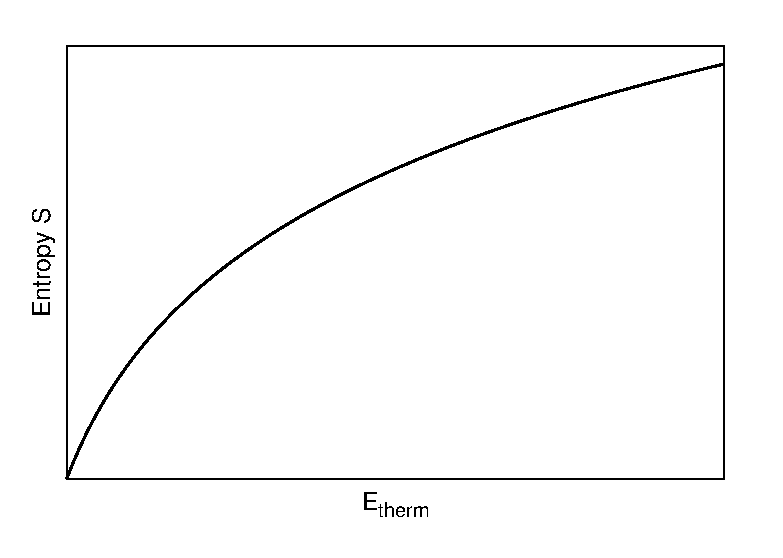
\includegraphics[width=3.5in]{second_law_and_entropy/entropy_vs_energy}
\caption{Entropy as a function of thermal energy.}
\label{fig:entropy_vs_energy}
\end{center}
\end{figure}

Now let's couple two subsystems, $A$ and $B$.  The combined energy is
fixed, $E_\text{total} = E_A + E_B$.  Consequently, as system $A$
gains energy, system $B$ loses energy, and vice-versa.  In
Fig.~\ref{fig:coupled_systems} we plot both $S_A$ and $S_B$, but
notice that the $S_B$ curve is flipped over left to right.  This is
because $E_B=0$ occurs at the right side of the plot, where $E_A$ is
at its maximum, and $E_B$ increases as you move to the left.  The
reason for plotting it this way is that we can, for a particular
choice of $E_A$, read off both $S_A(E_A)$ and $S_B(E_B)$.  Also shown
on the plot is the combined entropy $S_\text{total}=S_A+S_B$.


\begin{figure}
\begin{center}
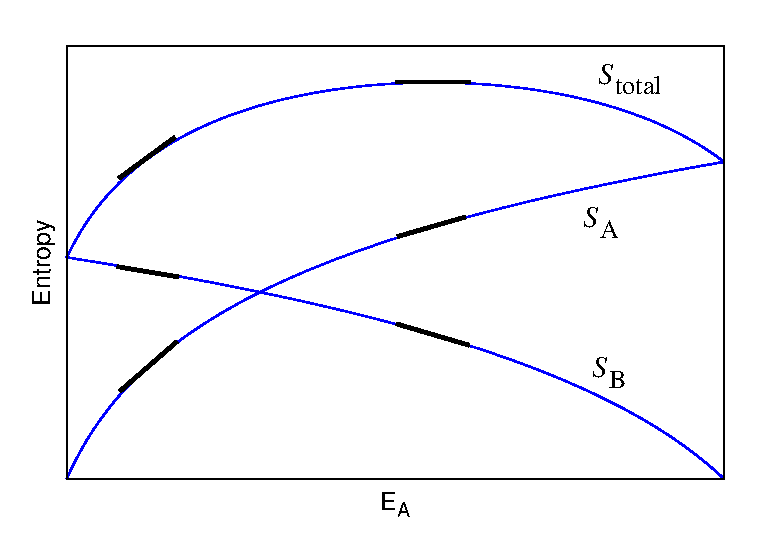
\includegraphics[width=4.5in]{second_law_and_entropy/coupled_systems.eps}
\caption{Entropies of subsystems $A$ and $B$, as well as the combined
system entropy $S_\text{total}$, all plotted versus $E_A$.}
\label{fig:coupled_systems}
\end{center}
\end{figure}

Now imagine starting with a relatively small value of $E_A$, where the
heavy lines are drawn on the left.  What would be the net effect on
the entropy if we were to take some energy from system $B$ and give it
system $A$?  The plot shows that $S_B$ would decrease and $S_A$ would
increase.  The plot also shows that, since the $S_A$ curve in this
region is steeper than the $S_B$ curve, system $A$ would gain 
more entropy than system $B$ would lose.  In other words,
$S_\text{total}$ would increase.  Therefore, the ``force'' of
probability pushing towards a (vastly) more probable state dictates
that energy flows from system $B$ to system $A$.

What the previous analysis should make clear is that the question of
which way the energy will flow is determined by the magnitude of the
{\it slope\/} on an entropy versus energy graph.  Whichever system,
$A$ or $B$, has the steeper slope will be the one to receive the
energy.

Let's carry this analysis further.  After some energy has flowed from
$A$ to $B$, we find that $E_A$ has increased to where the second set
of heavy lines are drawn.  Here, the slopes of the $S_A$ and $S_B$
curves are equal in magnitude and opposite in sign.  Any entropy
change of system $A$ is canceled by the entropy change of system $B$,
so there is no longer entropy gained by increasing $E_A$ (or
decreasing it).   Thermal energy will no longer be transferred because
we are at the maximum combined entropy, which can be seen from the
plot of $S_\text{total}$, and we have reached thermal equilibrium.
Any additional transfer of energy (in either direction) will
result in a decrease in total entropy.

All this discussion leads to the notion that the slope
$dS/dE_\text{therm}$ is directing the thermal energy traffic.
Whichever subsystem has the smaller slope will give up energy to the
subsystem which has the larger slope.  Hence, we define temperature as

\boxiteq{
\begin{equation}
\frac{1}{T} \equiv \frac{dS}{dE_\text{therm}},
\label{eq:temperature_def}
\end{equation}}

\noindent and our probability analysis becomes equivalent to the Clausius
statement.

This definition, then, explains the role of temperature in the second
law, but does it match our previous notions of temperature?  And what
does it mean intuitively?  First, yes, it does match the ideal gas
temperature, etc.  This can be shown by deriving the equipartition
theorem from this definition of temperature; all our previous uses for
temperature (such as the ideal gas) had their origin in the
equipartition theorem.

As for an intuitive meaning, think of it this way: inverse temperature
(that is, $1/T$) is a measure of how much use a system has for
energy.  When a system can find many ways to divide up the energy,
then adding some energy will increase $S$ a lot.  That is a low
temperature system.  A high temperature system is one where
diminishing returns has set in, and additional energy does not result
in a substantial entropy increase.

Finally, note that for large systems we can add some amount of energy
without significantly changing the temperature (for example, adding 10
joules of thermal energy to a cup of water).  In this case, we can
approximate Eq.~(\ref{eq:temperature_def}) as
\begin{equation}
\frac{1}{T} \approx \frac{\Delta S}{\Delta E_\text{therm}} 
\qquad\text{or}\qquad
T \approx  \frac{\Delta E_\text{therm}}{\Delta S}.
\label{eq:temperature_approx}
\end{equation}
This is often a handy way to {\em estimate} temperature from entropy change
or vice-versa.

\begin{example}{The Temperature of my Coffee}
Adding $50\units{J}$ of thermal energy to my coffee cup caused its
entropy to increase by an amount of $0.17\units{J/K}$.  Estimate the
temperature of my coffee.
\solution
According to Eq.~(\ref{eq:temperature_approx}) we have
\begin{equation}
T \approx  \frac{\Delta E_\text{therm}}{\Delta S} = 
\frac{50\units{J}}{0.17\units{J/K}} = 294\units{K}.
\end{equation}
That's room temperature.  Yuck!
\end{example}

\newpage

\section*{Problems}
\markright{PROBLEMS}

\begin{problem}
Consider an Einstein solid with three oscillators and four units of
energy.
\begin{enumerate}
\item Calculate the multiplicity for this macrostate.
\item Write out the triplet for each possible microstate.  For
  example, the microstate where the first oscillator has all the units
  of energy can be written as $(4,0,0)$.  Confirm that you find the
  correct number of microstates.
\end{enumerate}
\label{prob:multiplicityforthree}
\end{problem}

\begin{problem}
Calculate the multiplicity of an Einstein solid with 24 oscillators
and 15 energy units.  
\label{prob:mult_of_twentyfour}
\end{problem}

\begin{problem}
Suppose you roll a fair six-sided die three times in a row.
\begin{enumerate}
\item Determine the probability of getting exactly the sequence 1--3--2?
\item Now determine the probability of getting any other particular
sequence (hint: no calculation necessary).
\item What is the probability of rolling a sum of 6?
\end{enumerate}
\label{prob:rolldie}
\end{problem}

\begin{problem}
  For two Einstein solids with $N_A=3$ and $N_B=3$ and six energy
  units, how many times more probable is the macrostate with equally
  shared energy than the macrostate where system $A$ has all the
  energy?  Use Table~\ref{table:two_systems}.
\label{prob:twosolids}
\end{problem}

\begin{problem}
Is it really true that the entropy of an isolated system consisting of
two Einstein solids never decreases?  Consider a pair of very small
solids.  Explain why this statement is more accurate for large systems
than for small systems.
\end{problem}

\begin{problem}
A large object's entropy is observed to increase by $0.15\units{J/K}$
when we add $45\units{J}$ of thermal energy.  Assume that this causes
a negligible increase in the temperature of the object.  Determine
the approximate temperature of the object.
\label{prob:tempoflargeobject}
\end{problem}

\begin{problem}
  The idea of ``diminishing returns'' says that while the entropy does
  increase with increasing thermal energy, the slope is decreasing
  (see Fig.~\ref{fig:entropy_vs_energy}).  The Einstein solid
  multiplicity, like most materials, shows this behavior.  Here is how
  to see it:
  \begin{enumerate}
  \item For an Einstein solid with 10 oscillators and 5 energy units,
    calculate how much the entropy increases, i.e. $\Delta S$, if you
    add one more energy unit (you may leave your answer in terms of
    $k_B$).
  \item Now consider an Einstein solid with 10 oscillators and 15
    energy units, and calculate how much the entropy increases if you
    add one more energy unit.
  \item Do your answers to (a) and (b) confirm the diminishing
    returns?  Explain why.
\end{enumerate}
\label{prob:diminishing}
\end{problem}

\begin{problem}
For two Einstein solids $A$ and $B$, the entropy as a function of
thermal energy is given by 
\[
S_A= k_B\, 400\ln(E_A/300) \qquad S_B = k_B\, 100\ln(E_B/800)
\]
where $E_A$ and $E_B$ are the thermal energies of systems $A$ and
$B$.  If the two solids are brought to thermal equilibrium, what
relation, if any, can be made between the final energies $E_{A,f}$ and
$E_{B,f}$? 
\label{prob:entropyoftwosolids}
\end{problem}

\begin{problem}
Consider a very strange system whose multiplicity is $\Omega_A=1$
regardless of how much energy it has.  Imagine starting this system
with some amount of energy and bringing it into thermal contact with
system $B$, an Einstein solid.
\begin{enumerate}
\item In which direction will the energy flow, or will no energy flow?
\item What can you say about the energies of the final state?  For
  example, will they be equal?  If they are unequal, which is larger?
  Is there anything more you can conclude?
\end{enumerate}
\label{prob:strangesystem}
\end{problem}

%\begin{problem}
%The multiplicity of a monatomic ideal gas is given by $\Omega =
%c(E_\text{therm})^{3N/2}$, where $c$ is some constant that depends on
%the number of particles and volume, but does not depend on
%$E_\text{therm}$.  (Note: we will derive this result in
%Chapter~\ref{chapter:heat_engines}.) 
%\begin{enumerate}
%\item Use this multiplicity to find the entropy of an ideal gas.
%\item Use your result from part (a) and the definition of temperature
%  to derive the relation $E_\text{therm}=\frac{3}{2}Nk_BT$.  Hint: use
%  the logarithm properties $\ln(xy) = \ln x + \ln y$ and $\ln(x^n) =
%  n\ln x$.
%\end{enumerate}
%\end{problem}
%
%\begin{problem}
%There is no problem 10.
%\end{problem}

\begin{problem}
A substance has entropy $S=c\sqrt{E_\text{therm}}$, where $c$ is
  some constant.  Use the definition of temperature to find
  $E_\text{therm}$ as a function of $T$.
\end{problem}

\begin{problem}
Consider two Einstein solids with $N_A=3$ and $N_B=3$ and eight energy
units. 
\begin{enumerate}
\item Make a table like Table~\ref{table:two_systems}.  Note that many
  of the multiplicities you will need are already in
  Table~\ref{table:two_systems}, so there is no need to re-calculate
  everything. 
\item How many times more probable is the macrostate with equally
  shared energy than the macrostate where system $A$ has all the energy?
\end{enumerate}
\end{problem}

\begin{problem}
An Einstein solid has four oscillators and three units of energy.
\begin{enumerate}
\item Calculate the multiplicity of the solid.
\item Identify all the possible microstates using the parenthesis
  notation of Example~\ref{example:multiplicity}.
\end{enumerate}
\end{problem}

\begin{problem}
System $A$ and system $B$ are both large.    For system $A$, adding
$250\units{J}$ of thermal energy causes an entropy increase of
$0.80\units{J/K}$.  For system $B$, adding $250\units{J}$ of thermal
energy causes an entropy increase of $0.60\units{J/K}$.
\begin{enumerate}
\item Without mentioning temperature, use probability arguments to
  determine which way thermal energy will flow when systems $A$ and
  $B$ are thermally coupled.
\item Estimate the temperature of each object and check that your
  result is consistent with part (a).
\end{enumerate}
\end{problem}

\begin{problem}
Show that $S_{AB} = S_A + S_B$ follows from the definition of entropy.
\label{problem:entropy_additive}
\end{problem}

%\begin{problem}
%To get an idea of what the logarithm does to the definition of 
%entropy, let's try a simple calculation.  
%\begin{enumerate}
%\item Assume that you have
%a multiplicity $\Omega = 10^{10}$.  Take the natural log
%of this multiplicity and write down the entropy (as a multiple
%of Boltzmann's constant $k_B$) to five decimal places, i.e., 
%``S = ??.?????$k_B$.''
%Now, subtract 1 from your multiplicity (i.e. 9999999999) and take the natural
%log of that, and write it down the new entropy (as a multiple
%of $k_B$) to five decimal places.  Is there
%a noticeable drop in entropy due to the small drop in multiplicity?
%\item Repeat part (a), but this time subtract 10 from the multiplicity.
%Then do it again, subtracting 100, 1000, etc, until you finally
%see an entropy decrease that is noticeable to five decimal
%places.
%\item Write a few sentences explaining why total entropy is never
%observed to decrease in a real system (with $N \approx 10^{23}$),
%even though the multiplicity {\bf can} decrease slightly.
%\end{enumerate}
%\label{prob:natural_log}
%\end{problem}

\begin{problem}
Entropy applies to more than just heat flow.  We can use entropy
and the second law of thermodynamics to discuss movement of
air in a room.
\begin{enumerate}
\item Consider a room with only 100 gas molecules.  Theoretically,
the gas molecules can move anywhere in the room.  Calculate the 
probability that all 100 of the molecules will be found on
one particular side of the room.
\item Now, consider a real room with a realistic amount of gas in
it -- let's say that there are $10^{26}$ gas molecules in the room.
Calculate the probability that all of these gas molecules will
be found in one particular side of the room.  (Note:  the probability
is {\bf so} small that your calculator or computer might simply
give ``0'' for the answer.)
\item Is it reasonable to say that you will ``never'' find all the
air in one side of the room?
\item Now, write a couple of sentences explaining why it is
(from a probability perspective) that when a perfume bottle is
opened, the scent of the perfume will spread throughout
the room.  
\item After the perfume smell has spread throughout the room,
would you expect all of the perfume molecules to go back
into the bottle?  Discuss this using the entropic form of the
second law of thermodynamics.
\end{enumerate}
\end{problem}
\newpage

\begin{problem}
The graphs in the figure below give plots of entropy $S$ vs.\ $E_\text{therm}$ for
two different solids, A and B.  Solid A starts with indicated energy $E_A$ and 
entropy $S_A$, and Solid B starts with $E_B$ and $S_B$.  
When Solid A has energy $E_A$, the slope of the entropy 
vs.\ energy curve is $dS_A/dE= 0.2\units{K$^{-1}$}$, and 
when Solid B has energy $E_B$, the slope of the entropy vs.\ energy 
curve is $dS_B/dE = 0.4\units{K$^{-1}$}$.

\begin{figure}[h]
\begin{center}
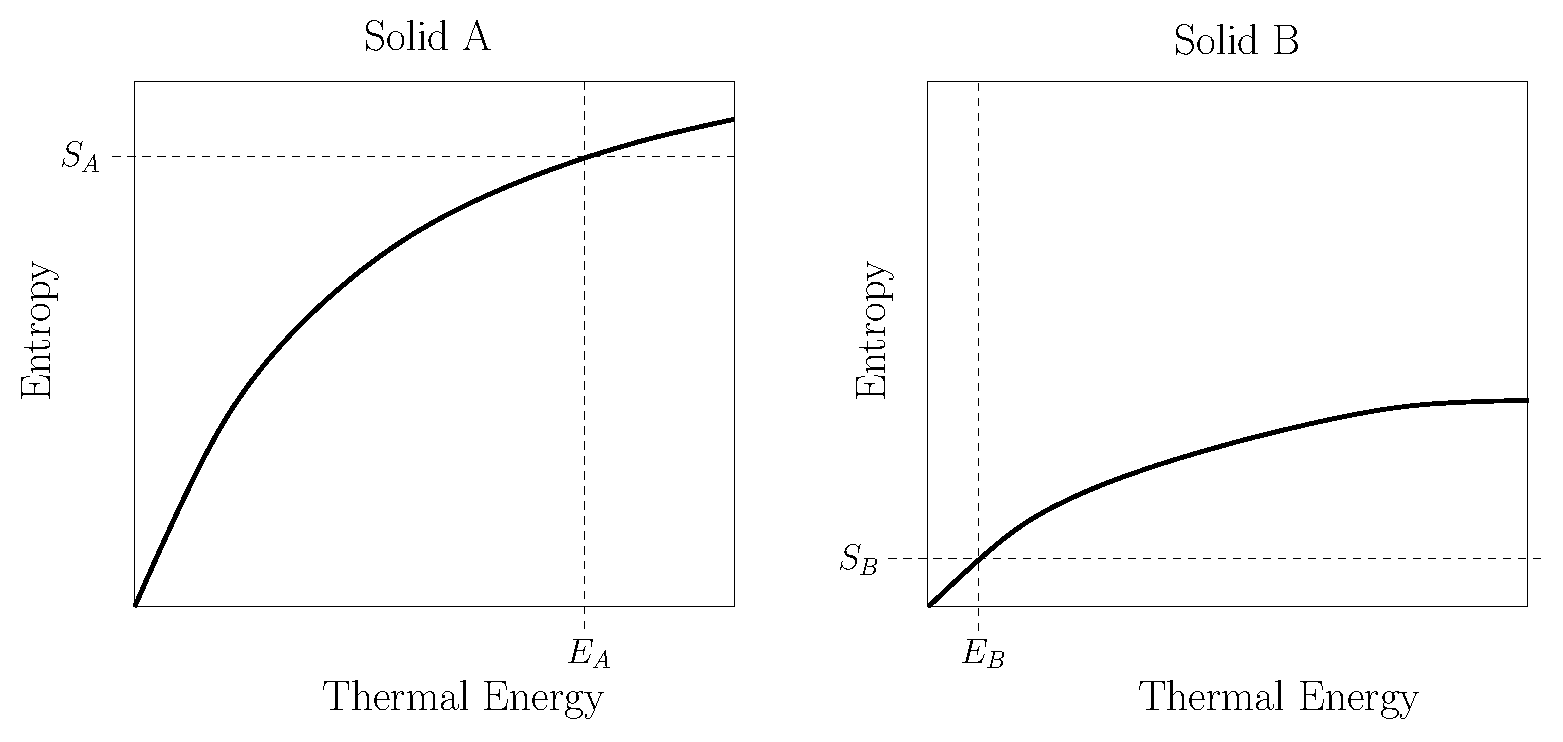
\includegraphics[width=5.0in]{second_law_and_entropy/energy_transferA.eps}
\caption{Figure for Problem \ref{prob:energy_transferA}}
\label{fig:energy_transferA}
\end{center}
\end{figure}

The two solids are brought into thermal contact with each other so that
energy can flow between them.
\begin{enumerate}
\item Which way will the energy flow:  from A to B, from B to A, or 
will no energy flow?  Give  qualitative reasoning to support your answer.
\item Now let's get quantitative.  Calculate the approximate  
entropy changes $\Delta S_A$ and $\Delta S_B$, and $\Delta S_\text{total}$ 
if $3\units{J}$ of energy flow between the two solids in the direction 
that you chose in part (a).  
\item By what factor has the multiplicity for the total system increased
from this energy transfer?  In other words, calculate the ratio of 
multiplicities $\Omega_\text{after}/\Omega_\text{before}$.

Note:  The answer you get will be a ridiculously, mind-boggling,
impossible-to-put-into-words-just-how-huge-it-really-is number
that you will not be able to calculate ---  you'll have to express it as
$e^\text{something really big}$.  To give you and idea of just how
large this number is, if you were to write it as a digit followed by a
bunch of zeros, and if each digit were $5\units{mm}$ wide, the number
would fill up several {\em light years}.

\item Explain in your own words why heat flows in this system when the
two solids are brought into contact.  Don't use the words ``entropy''
or ``second law'' but rather explain it based on probabilities.

\end{enumerate}
\label{prob:energy_transferA}
\end{problem}

\begin{problem}
The graphs in the figure below give plots of entropy $S$ vs.\
$E_\text{therm}$ for two different solids, A and B.  Solid A starts with
indicated energy $E_A$ and entropy $S_A$, and Solid B starts with $E_B$
and $S_B$.  When Solid A has energy $E_A$, the slope of the entropy vs.\
energy curve is $dS_A/dE= 0.5\units{K$^{-1}$}$, and when Solid B has
energy $E_B$, the slope of the entropy vs.\ energy curve is $dS_B/dE =
0.1\units{K$^{-1}$}$.

\begin{figure}[h]
\begin{center}
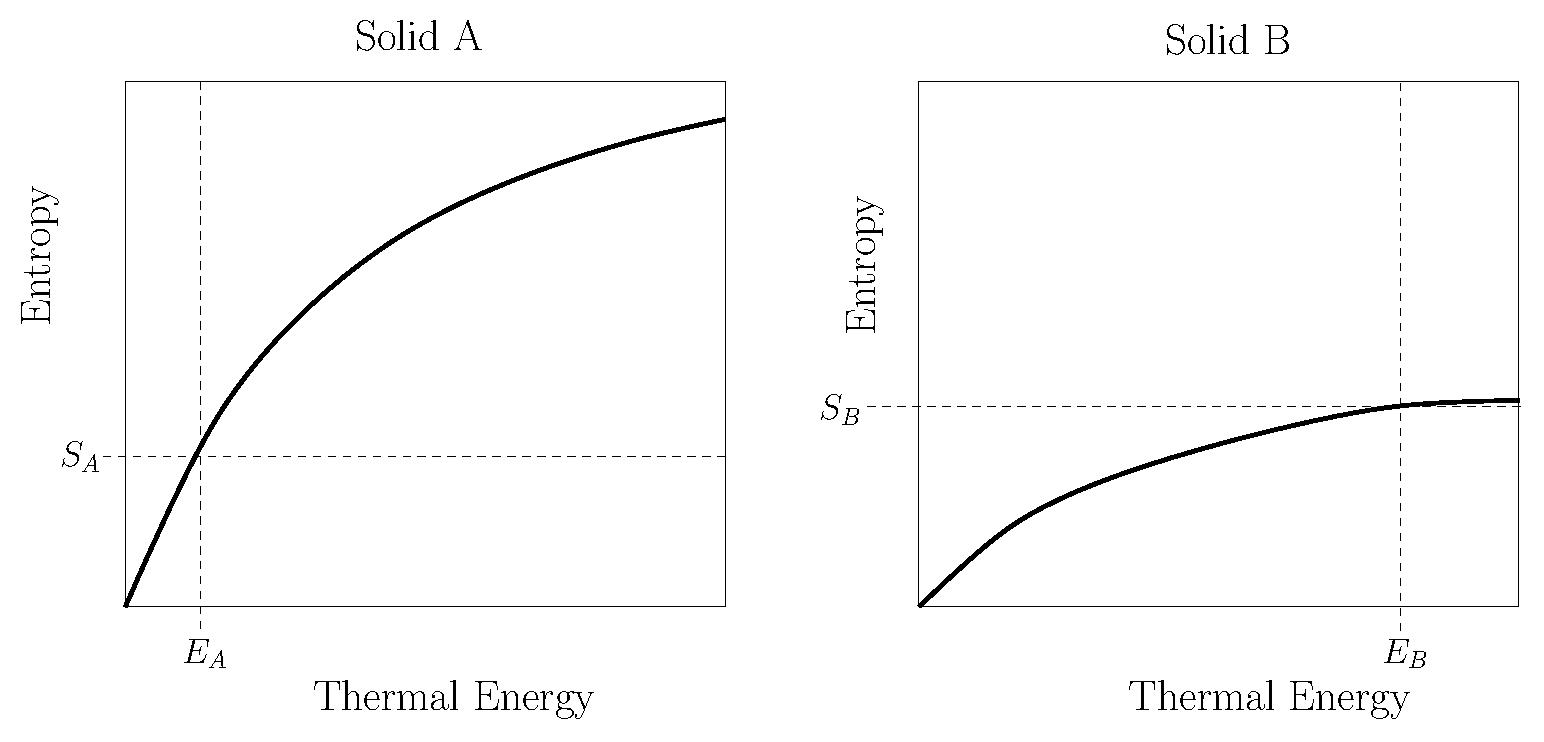
\includegraphics[width=5.0in]{second_law_and_entropy/energy_transferB.eps}
\caption{Figure for Problem \ref{prob:energy_transferB}}
\label{fig:energy_transferB}
\end{center}
\end{figure}

The two solids are brought into thermal contact with each other so that
energy can flow between them.
\begin{enumerate}
\item Which way will the energy flow:  from A to B, from B to A, or 
will no energy flow?  Give  qualitative reasoning to support your answer.
\item Now let's get quantitative.  Calculate the approximate  
entropy changes $\Delta S_A$ and $\Delta S_B$, and $\Delta S_\text{total}$ 
if $2\units{J}$ of energy flow between the two solids in the direction 
that you chose in part (a).  
\item By what factor has the multiplicity for the total system increased
from this energy transfer?  In other words, calculate the ratio of 
multiplicities $\Omega_\text{after}/\Omega_\text{before}$.

Note:  The answer you get will be a ridiculously, mind-boggling,
impossible-to-put-into-words-just-how-huge-it-really-is number
that you will not be able to calculate ---  you'll have to express it as
$e^\text{something really big}$.  To give you and idea of just how
large this number is, if you were to write it as a digit followed by a
bunch of zeros, and if each digit were $5\units{mm}$ wide, the number
would fill up several {\em light years}.

\item Explain in your own words why heat flows in this system when the
two solids are brought into contact.  Don't use the words ``entropy''
or ``second law'' but rather explain it based on probabilities.

\end{enumerate}
\label{prob:energy_transferB}
\end{problem}


\newpage


\newpage
\begin{problem}
System A and System B are brought into thermal contact when the energy in
A is $E_A= 1000\units{J}$ and the energy in B is $E_B=1100\units{J}$.
Using the table below, listing energies and corresponding entropies of
the two systems, determine whether heat will flow from A to B, or 
from B to A.  Show all your work.

\begin{center}
{\large
\renewcommand{\arraystretch}{1.8}
\begin{tabular}{|c|c|c|c|} \hline
$E_A$ (J) & $E_B$ (J)  & $S_A$ (J/K) & $S_B$ (J/K)
     \\ \hline \hline
    950   &       1150   &     6.76     &    10.34     \\ \hline
    975   &       1125   &     6.84     &    10.21     \\ \hline
{\bf 1000}&  {\bf 1100}  & {\bf 6.93}   & {\bf   10.08} \\ \hline
    1025   &      1075   &     7.02     &     9.95     \\ \hline
    1050   &      1050   &     7.10     &     9.82     \\ \hline
\end{tabular}
\renewcommand{\arraystretch}{1.0}
}
\end{center}
\end{problem}

%\begin{problem}{Strategic Studying}
%(Problem under development.)
%Imagine that a physics test is imminent, and you have exactly 200 minutes
%left to prepare for the test.  The test has two parts: 60 points for
%questions about classical mechanics relativity, and 40 points for
%questions about relativity.  The graphs below represent the number of
%points you expect to get on each part of the test vs.\ the amount of
%time you put into studying.
%\end{problem}

